\documentclass[12pt]{article}
% Adaptado de C:/GitHub/Mestrado/Template/Template.tex.
\usepackage[T1]{fontenc}
\usepackage[utf8]{inputenc}
\usepackage[brazilian]{babel}
\usepackage{graphicx,booktabs,array,amsmath,amssymb,microtype}
\usepackage{geometry}
\usepackage{pdflscape,caption,float,placeins,longtable,needspace}
\geometry{a4paper,margin=2.5cm}
\usepackage{parskip,csquotes}
\interfootnotelinepenalty=10000
\usepackage[backend=biber,style=abnt]{biblatex}
\addbibresource{references.bib}
\usepackage{hyperref}
\hypersetup{colorlinks=true,urlcolor=blue,linkcolor=blue,citecolor=blue}
\newcommand{\instituicao}{UNIVERSIDADE FEDERAL DE SANTA CATARINA}
\newcommand{\departamento}{Programa de Pós-Graduação em Economia}
\newcommand{\curso}{Mestrado}
\newcommand{\disciplina}{Desigualdade, Diversidade e Redes}
\newcommand{\titulo}{Da produção à demanda}
\newcommand{\subtitulo}{Estrutura da rede intersetorial de atribuição de CO\textsubscript{2} no Brasil e implicações para a coordenação da mitigação}
\newcommand{\autor}{Gabriel Pincelli Cintra}
\newcommand{\local}{Florianópolis}
\newcommand{\dataentrega}{21 de outubro de 2026}
\newcommand{\imprimirtitulodois}{
\begin{center}
  {\Large\bfseries\MakeUppercase{\instituicao}\par}
  \vspace{0.2em}{\large \departamento\par}
  \vspace{0.2em}{\normalsize\textbf{\disciplina}\ (\curso)\par}
  \vspace{1.4em}{\LARGE\bfseries \titulo\par}
  \vspace{0.25em}{\large\itshape \subtitulo\par}
  \vspace{1.5em}
\end{center}
\noindent\begin{minipage}{0.48\textwidth}
  \raggedright\normalsize \autor
\end{minipage}\hfill
\begin{minipage}{0.48\textwidth}
  \raggedleft\normalsize \local, \dataentrega
\end{minipage}
\vspace{1.0em}\hrule\vspace{1.0em}}
% Figuras do corpo compartilham páginas com a narrativa.
\renewcommand{\topfraction}{0.80}
\renewcommand{\bottomfraction}{0.80}
\renewcommand{\textfraction}{0.12}
\setcounter{topnumber}{1}
\setcounter{bottomnumber}{1}
\captionsetup{font=small}
\begin{document}
\imprimirtitulodois
\begin{abstract}
Este artigo examina como relações intersetoriais conectam as emissões atribuídas pela produção e pela demanda no Brasil. Combina a MIP de 2015, com 67 atividades, a intensidades aproximadas de CO\textsubscript{2}, distinguindo volume, presença como fornecedor e concentração das atribuições. A rede é quase completa, mas seus pesos são desiguais. Energia distribui emissões entre diversos produtos finais; construção reúne emissões de outras origens e mantém elevada atribuição à própria atividade. O filtro de disparidade retém 13,40\% das ligações e 70,69\% do peso intersetorial, com cobertura desigual entre perfis. A análise identifica relações a investigar conjuntamente para mitigação, sem estimar efeitos de políticas. Os resultados ambientais são condicionais às intensidades utilizadas.
\end{abstract}

\section{Introdução}

As mesmas emissões de dióxido de carbono (CO\textsubscript{2}) podem produzir distribuições setoriais distintas conforme o critério de atribuição. Pela produção, são contabilizadas na atividade em que ocorrem; pela demanda, são associadas ao setor do produto final, considerando sua cadeia de produção. As emissões da geração de eletricidade, por exemplo, podem ser registradas no setor elétrico ou atribuídas aos produtos finais cuja produção requer essa eletricidade. Comparar essas perspectivas ajuda a relacionar os setores emissores às demandas que mobilizam sua produção \parencite{marques2012,millerBlair2009}.

Este trabalho pergunta: \textbf{quais relações intersetoriais compõem as diferenças entre as emissões atribuídas pela produção e pela demanda na economia brasileira de 2015, e como essas relações se organizam em termos de volume, concentração e conectividade?} O objetivo é caracterizar essa estrutura e discutir suas implicações para identificar oportunidades de coordenação da mitigação. Utiliza-se a Matriz de Insumo-Produto (MIP) nacional de 2015, com 67 atividades \parencite{ibge2015mip}, combinada com coeficientes setoriais de emissão.

Os totais setoriais não mostram, isoladamente, como as origens emissoras se relacionam aos produtos finais. Uma pegada elevada pode concentrar-se em poucas origens ou distribuir-se entre muitas; um grande emissor pode atender a demandas finais de diferentes atividades. Além disso, um setor pode apresentar uma diferença pequena entre as contas e, ao mesmo tempo, ter grandes volumes de emissões próprias atribuídas a outros produtos finais e de emissões de outras atividades atribuídas aos seus produtos finais. Identificar as contrapartes e a distribuição dos pesos permite distinguir esses perfis, além de comparar suas posições nos rankings de emissões.

A proposta articula a contabilidade ambiental à análise de redes ponderadas. \textcite{millerBlair2009} fundamentam o modelo insumo-produto e a extensão ambiental que relaciona produção e demanda final. \textcite{sanguinetAzzoni2024} examinam emissões nas cadeias produtivas regionais brasileiras sob diferentes perspectivas de atribuição. No campo das redes, \textcite{huang2019} constroem uma rede de emissões para a China e combinam filtragem de ligações, indicadores de posição e comunidades. Este trabalho adapta a representação de atribuição e a seleção de ligações ao recorte nacional brasileiro, com foco na relação entre as contas pela produção e pela demanda.

A contribuição pretendida é identificar quais contrapartes compõem as diferenças entre as duas contas e se as relações de atribuição se concentram em poucas atividades ou se distribuem entre muitas. A análise tem caráter descritivo e exploratório. Na representação em rede, as atividades são os nós e as ligações dirigidas associam origens emissoras a produtos finais, com pesos dados pelos volumes de emissões atribuídos. Serão examinados os volumes, a concentração dos pesos e a conectividade de uma rede reduzida por um critério explícito de seleção de ligações, denominada \textit{backbone}. Para essa seleção, será avaliado o filtro de disparidade de \textcite{serrano2009}. As medidas de concentração serão calculadas antes da filtragem, pois o número de ligações selecionadas não representa, por si só, a diversidade das relações originais.

O recorte abrange emissões da produção nacional associadas à demanda doméstica e às exportações, excluindo emissões estrangeiras. Os coeficientes de \textcite{sanguinetAzzoni2024} constituem a referência inicial de um cenário exploratório, com validação ambiental e monetária pendente, detalhada na seção~\ref{sec:dados}. Por isso, o trabalho ainda não sustenta rankings definitivos de emissores brasileiros.

A discussão de política se concentrará em conjuntos de setores e demandas que mereçam investigação conjunta. Intervenções nos processos produtivos e no uso de energia e materiais ao longo das cadeias são frentes complementares de mitigação discutidas por \textcite{rissman2020}. A rede poderá informar quais relações examinar, mas não estimará a eficácia ou o custo de instrumentos de política.

As seções seguintes apresentam os dados, desenvolvem a metodologia, expõem os resultados e discutem suas implicações e limitações, encerrando com as conclusões.

\section{Dados e método}
\label{sec:dados}
A base econômica é a MIP brasileira de 2015, com 67 atividades e valores em milhões de reais a preços básicos \parencite{ibge2015mip}. A fronteira abrange emissões nacionais associadas à demanda doméstica e às exportações; exclui emissões estrangeiras. O destino identifica o setor do produto final, não seu comprador imediato ou país consumidor. A conta pela demanda não equivale à pegada mundial do consumo dos residentes.

As intensidades diretas de \textcite{sanguinetAzzoni2024}, em Gg de CO\textsubscript{2}/R\$ milhão de produção, são interpoladas entre 2011 e 2018, com pesos $3/7$ e $4/7$. Trata-se de uma aproximação: a evolução linear, a compatibilidade de preços e a alocação ambiental setorial limitam sua interpretação. A documentação de preparação e as verificações encontram-se no Apêndice~\ref{ap:metodo}; os resultados não representam um inventário físico validado de 2015.

O modelo parte dos coeficientes técnicos $A$, da inversa de Leontief $L=(I-A)^{-1}$, da demanda final $y$ e das intensidades $\varphi$. A atribuição de emissões é
\begin{equation}
F=\operatorname{diag}(\varphi)L\operatorname{diag}(y),\qquad c=F\mathbf1,\quad u=F^\top\mathbf1.
\label{eq:artigo-F}
\end{equation}
Cada $F_{ij}$ representa emissões em $i$ atribuídas ao produto final de $j$, em Gg de CO\textsubscript{2}, incorporando requisitos diretos e indiretos. As contas $c$ e $u$ somam as mesmas emissões por origem e destino. O exemplo do Apêndice~\ref{ap:metodo} ilustra essa conservação. As arestas representam atribuições contábeis; concatená-las não reconstrói etapas produtivas.

Para comparar presença como fornecedor e magnitude ambiental, calcula-se $q_i=\sum_{j\ne i}L_{ij}$. Essa soma adimensional dá peso unitário à demanda de cada outro produto final, exclui a diagonal inteira e independe das intensidades ambientais. Não mede quantidade de clientes ou insubstituibilidade. A comparação com as participações em $c$ e $u$ distingue requerimentos padronizados de volumes associados à demanda observada.

A rede dirigida tem 67 nós e pesos $W_{ij}=F_{ij}$ para $i\ne j$, com diagonal zero. As forças externas de saída e entrada são $s_i^{out}=c_i-F_{ii}$ e $s_i^{in}=u_i-F_{ii}$. Sua diferença corresponde ao saldo $u_i-c_i$. A concentração é medida pelo número efetivo $D_2=1/\sum p^2$, em que $p$ representa as participações das contrapartes em cada força. Valores maiores indicam distribuição mais equilibrada; perfis nulos permanecem indefinidos.

O filtro de disparidade \parencite{serrano2009} seleciona relações cuja participação se destaca sob um modelo nulo de repartição aleatória da força. Aplica-se uma vez a $W$, retendo a ligação se o teste na origem ou no destino passa em $\alpha=0{,}05$, com sensibilidade a 0,01 e 0,10. O backbone preserva pesos originais; a cobertura mede a fração de peso retida globalmente e por perfil. As contas e a concentração permanecem calculadas antes do filtro.


\section{Resultados}
\label{sec:resultados}
\subsection{Panorama nacional das atribuições}

A matriz completa conecta os totais setoriais às relações que os compõem (Figura~\ref{fig:panorama-F}). As cores mostram as atribuições entre cada origem emissora e produto final; as margens somam essas relações pela produção e pela demanda. A diagonal permanece visível, distinguindo a atribuição ao próprio produto das relações entre atividades que serão examinadas na rede externa.

As duas contas totalizam 683,70 mil Gg de CO\textsubscript{2}, dos quais 392,92 mil Gg, ou 57,47\%, ficam na diagonal e 290,78 mil Gg entre atividades distintas. A conservação é uma identidade contábil; a repartição dos pesos é o objeto da análise. Por isso, uma atividade pode concentrar emissões próprias sem distribuir volume semelhante para outros produtos finais.

%TC:ignore
\begin{figure}[!htb]
\centering
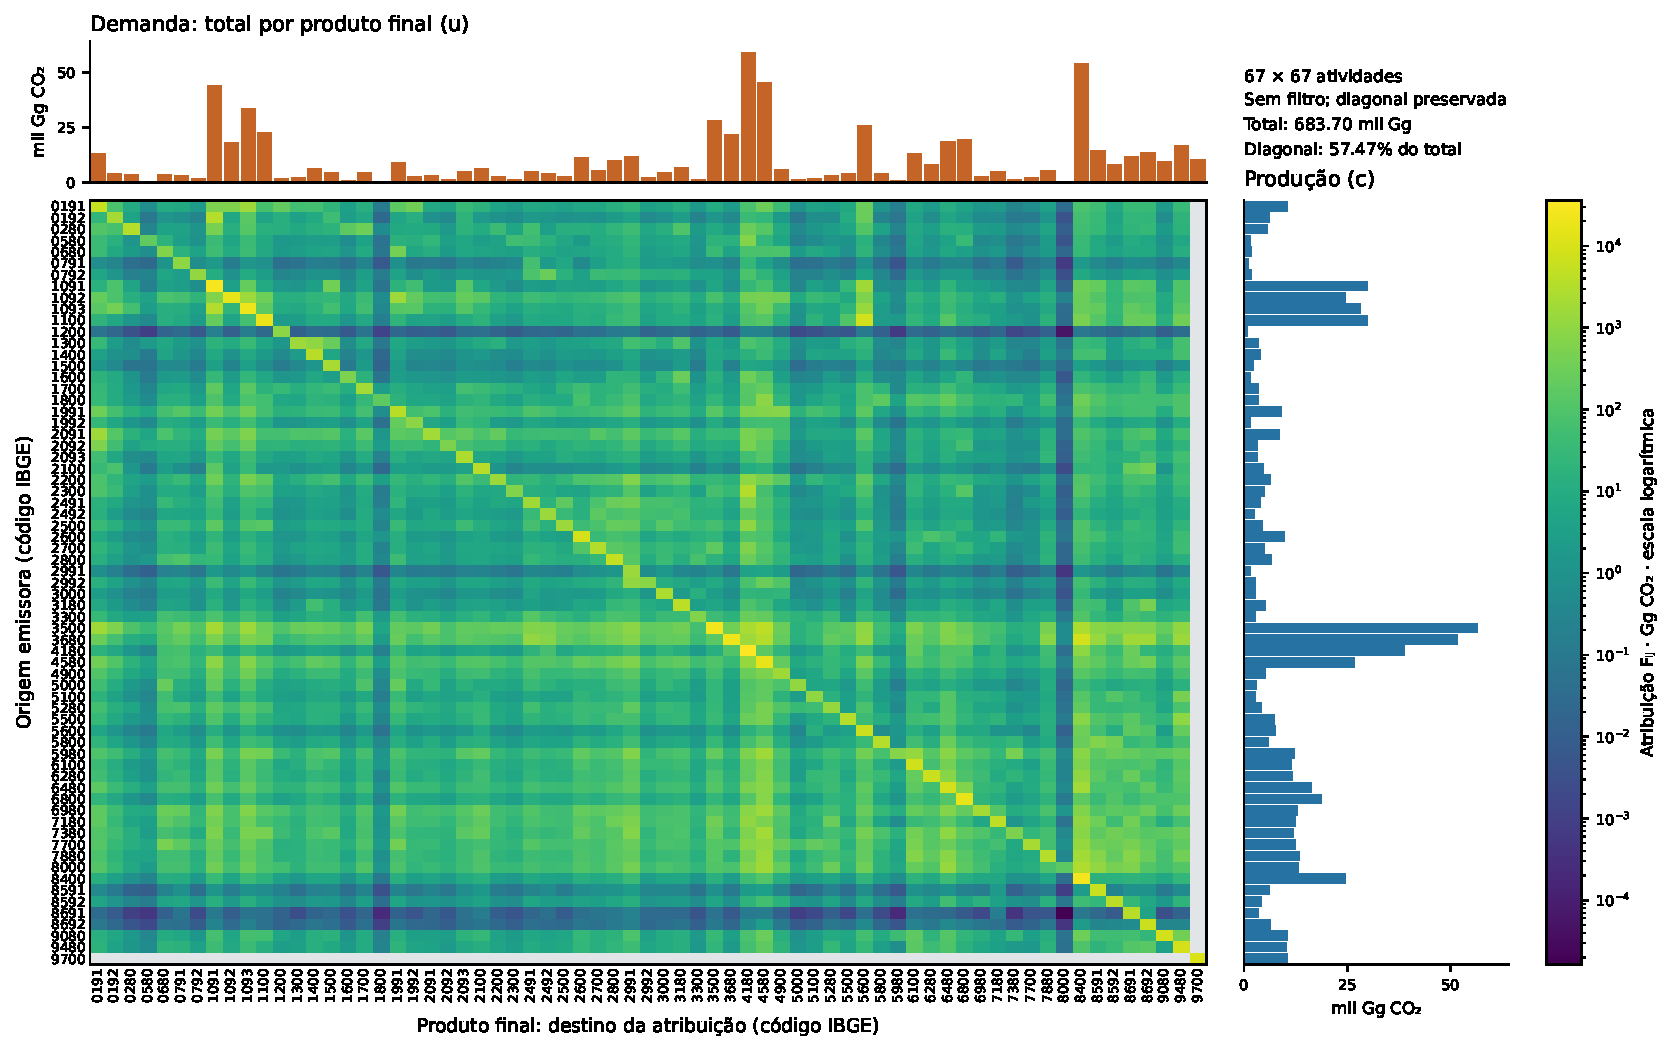
\includegraphics[width=\linewidth,height=0.55\textheight,keepaspectratio]{figuras/artigo_matriz_F.pdf}
\caption{Matriz nacional de atribuição de CO\textsubscript{2} e contas marginais, Brasil, 2015.}
\label{fig:panorama-F}
\begin{minipage}{\linewidth}\footnotesize
Fonte: elaboração própria, MIP do IBGE e intensidades aproximadas de Sanguinet e Azzoni (2024). Matriz $F$ integral: 67 origens emissoras nas linhas e 67 produtos finais nas colunas, na mesma ordem IBGE (códigos no Apêndice E). Cor em escala logarítmica dos pesos positivos, em Gg de CO\textsubscript{2}; cinza: zero. Não há filtro, agregação ou normalização por linha/coluna. A diagonal é preservada. Acima, soma das colunas ($u$, demanda); à direita, soma das linhas ($c$, produção). Barras em mil Gg, com escala linear de mesma amplitude. As duas contas preservam o mesmo total. As células representam atribuição direta e indireta, não transações imediatas.
\end{minipage}
\end{figure}
%TC:endignore

\subsection{Magnitude ambiental e presença produtiva}

As atividades mudam de posição ambiental sem alterar sua presença como fornecedoras. Na Figura~\ref{fig:emissao-fornecedor}, comércio, refino e transporte terrestre apresentam requerimentos elevados nas cadeias padronizadas; água e resíduos e construção combinam menor presença nessa comparação com participação relevante nas emissões próprias do cenário. Energia reúne participação emissora elevada e requerimentos inferiores aos dos três fornecedores destacados. Emitir muito e participar intensamente das cadeias dos demais produtos são dimensões relacionadas, mas distintas.

A passagem da produção à demanda evidencia o papel de construção como destino da atribuição. Sua participação sobe de 5,68\% para 8,69\%, enquanto a de energia cai de 8,28\% para 4,13\%. Comércio também ganha participação, de 3,91\% para 6,64\%. O deslocamento horizontal mantém a mesma estrutura econômica no eixo vertical: muda o critério aplicado às mesmas emissões. Esses contrastes descrevem o cenário adotado, não uma hierarquia ambiental independente da fonte.

%TC:ignore
\begin{figure}[!htb]
\centering
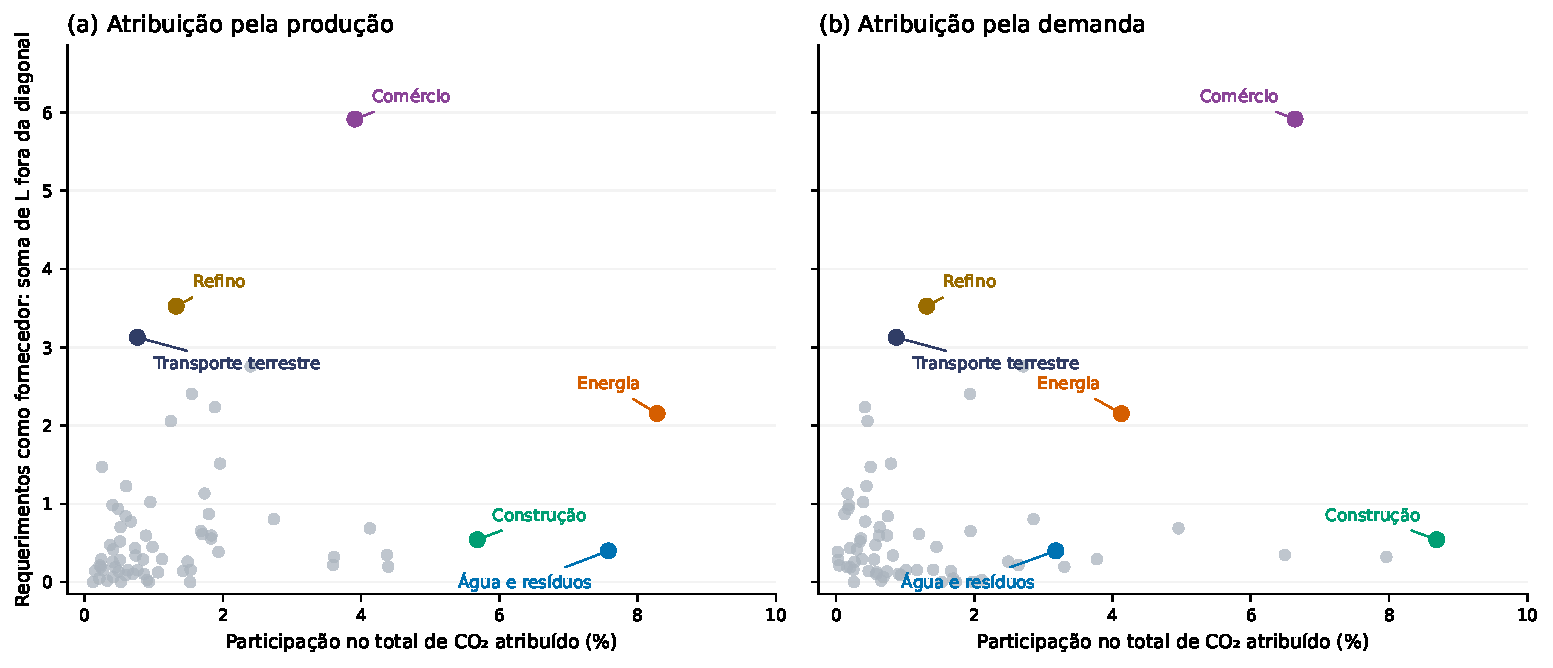
\includegraphics[width=\linewidth,height=0.55\textheight,keepaspectratio]{figuras/emissao_presenca_fornecedor.pdf}
\caption{Presença como fornecedor e participação nas contas pela produção e pela demanda.}
\label{fig:emissao-fornecedor}
\begin{minipage}{\linewidth}\footnotesize
Fonte: elaboração própria, MIP de 2015 e intensidades aproximadas de Sanguinet e Azzoni (2024). Todos os 67 setores, com escalas iguais. Eixo vertical: $q_i=\sum_{j\ne i}L_{ij}$, adimensional, sem diagonal e com peso unitário para cada outro destino. Eixo horizontal: participação percentual em $c$ (a) e $u$ (b), incluindo a diagonal de $F$. Os seis destaques retomam casos explorados anteriormente; não são uma classificação exaustiva. Sem filtragem de ligações.
\end{minipage}
\end{figure}
%TC:endignore

\subsection{Uma rede densa com pesos desiguais}

A rede contém quase todas as conexões possíveis, mas essa presença não descreve a distribuição dos volumes. São 4\,290 arestas, densidade de 97,01\% e 66 atividades conectadas em ambas as direções, com grau 65. Serviços domésticos é o único isolado externo. Os requisitos indiretos incorporados em $F$ contribuem para essa densidade; por isso, contar vínculos positivos pouco distingue os setores.

Os pesos externos se repartem de forma desigual: energia e água/resíduos têm saídas externas próximas, de 31,32 e 31,23 mil Gg, mas 20,79 e 9,88 destinos efetivos. Volumes semelhantes podem, portanto, corresponder a perfis com concentrações diferentes (Figura~\ref{fig:indicadores-resultados}).

O backbone reduz a quantidade de ligações com perdas desiguais de cobertura. Em $\alpha=0{,}05$, preserva 575 arestas, 13,40\% das originais, e 70,69\% do peso intersetorial. Entretanto, as medianas locais são 59,32\% nas saídas e 55,69\% nas entradas, com mínimos próximos de um terço. A cobertura agregada não garante representação igualmente completa de todos os setores. Nos parâmetros 0,01 e 0,10, retêm-se respectivamente 338 e 755 arestas, com 57,39\% e 77,35\% do peso; os detalhes estão no Apêndice~\ref{ap:sensibilidade}.

%TC:ignore
\begin{figure}[!htb]
\centering
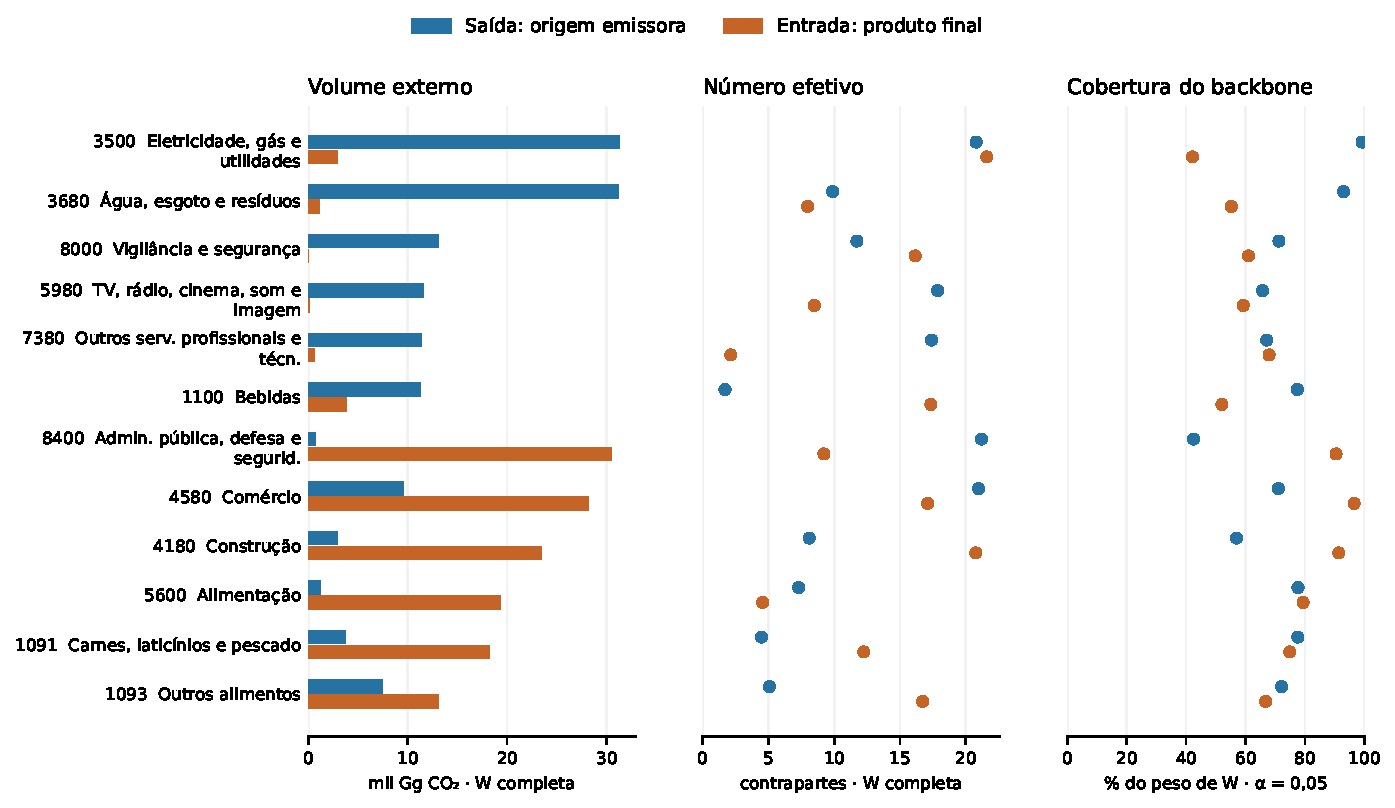
\includegraphics[width=\linewidth,height=0.55\textheight,keepaspectratio]{figuras/artigo_indicadores.pdf}
\caption{Volume, concentração e cobertura descrevem dimensões diferentes.}
\label{fig:indicadores-resultados}
\begin{minipage}{\linewidth}\footnotesize
Fonte: elaboração própria. União das seis maiores forças de saída e seis de entrada em $W$: 12 atividades, na ordem da seleção. Azul: saída da origem emissora; laranja: entrada no produto final. Volume em mil Gg de CO\textsubscript{2} e número efetivo calculados em $W$ completa, sem diagonal. Cobertura: peso retido no backbone de $\alpha=0{,}05$ dividido pela força da mesma atividade e direção. Não é cobertura do inventário ambiental.
\end{minipage}
\end{figure}
%TC:endignore

\subsection{Energia e construção: origens, destinos e contrapartes}

Energia distribui emissões para outros produtos, enquanto construção reúne atribuições de outras origens. Energia tem 56,62 mil Gg pela produção e 28,23 mil Gg pela demanda; suas saídas e entradas externas são 31,32 e 2,92 mil Gg. Construção apresenta 38,84 e 59,40 mil Gg nas contas completas, com 2,93 e 23,48 mil Gg externos. Sua pequena saída externa não significa baixa emissão própria: 35,91 mil Gg permanecem na diagonal.

As contrapartes tornam esses papéis concretos (Figura~\ref{fig:relacoes-focais}). Comércio, administração pública, construção e atividades alimentares aparecem entre os principais destinos externos de energia. Nas entradas de construção destacam-se minerais não metálicos, energia, água/resíduos e comércio. Energia $\rightarrow$ construção representa cerca de 2\,263 Gg, equivalentes a 7,2\% das saídas externas da origem e 9,6\% das entradas externas do destino. A mesma relação tem importância relativa diferente conforme a ponta examinada.

A seleção reflete essa assimetria local. Das 62 saídas retidas de energia, 56 passam somente pelo teste de entrada no destino: energia participa de forma saliente de muitas demandas, embora cada uma represente pouco de sua saída. Das 45 entradas retidas de construção, 41 passam somente pelo teste de saída na origem: construção se destaca entre os destinos dessas origens. A ligação entre energia e construção passa pelos dois testes. Esses motivos não equivalem a prioridades de mitigação.

A representação preserva melhor os sentidos predominantes. A cobertura chega a 99,2\% nas saídas de energia e 91,4\% nas entradas de construção, mas é de 42,1\% e 57,0\% nos sentidos inversos. A barra agregada das demais relações impede que a seleção visual das seis maiores seja confundida com o perfil completo. Mesmo com boa cobertura, 62 destinos retidos de energia e 45 origens de construção não medem diversidade: os números efetivos correspondentes em $W$ são próximos, ambos de 20,8.

%TC:ignore
\begin{figure}[!htb]
\centering
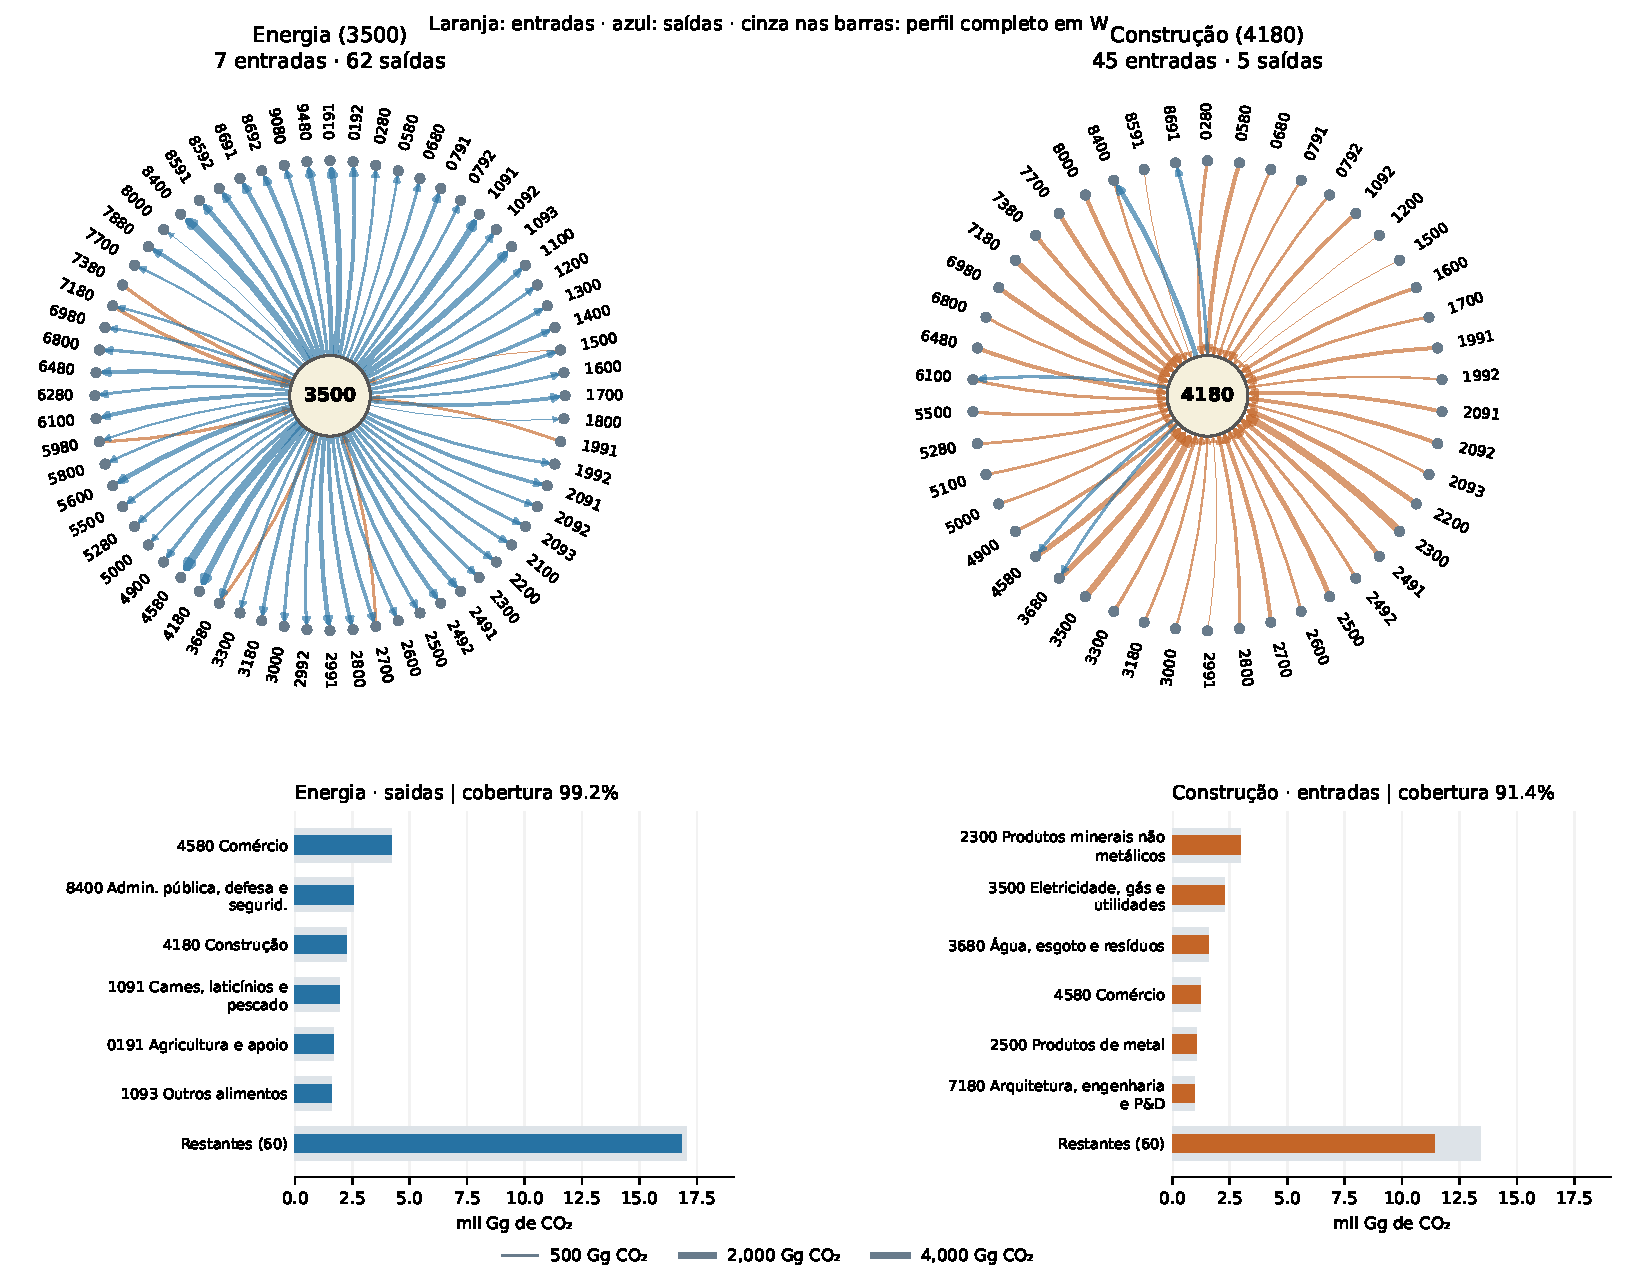
\includegraphics[width=\linewidth,height=0.55\textheight,keepaspectratio]{figuras/artigo_relacoes_combinada.pdf}
\caption{Contrapartes e cobertura dos perfis de energia e construção.}
\label{fig:relacoes-focais}
\begin{minipage}{\linewidth}\footnotesize
Fonte: elaboração própria. Acima: todas as relações incidentes a energia e construção no backbone de $\alpha=0{,}05$, sem diagonal; setas da origem emissora ao produto final. Azul: saídas; laranja: entradas; espessura proporcional à raiz do peso, com escala comum em Gg de CO\textsubscript{2}. Nós centrais identificam as atividades focais; demais códigos constam do Apêndice E. Posição circular sem interpretação econômica. Abaixo: saídas de energia e entradas de construção, com as seis maiores contrapartes em $W$ e soma das 60 restantes. Cinza: peso completo; cor: parcela retida, sem renormalização. Escala linear comum, em mil Gg de CO\textsubscript{2}. Cobertura relativa ao perfil inteiro. O agregado restante não representa uma atividade.
\end{minipage}
\end{figure}
%TC:endignore

\section{Discussão: relações para investigar conjuntamente}

A análise relacional complementa os rankings ao identificar quais origens e produtos finais compõem seus contrastes. A presença como fornecedor responde a demandas padronizadas; os volumes ambientais combinam estrutura produtiva, intensidade emissora e demanda observada. A concentração acrescenta como o volume se reparte, enquanto o backbone destaca relações sob uma regra local. Nenhuma dessas dimensões substitui as demais, e reunir indicadores não constitui confirmação independente de um mesmo resultado.

Os perfis de energia e construção sugerem diferentes escalas de coordenação. Uma origem associada a muitos produtos finais motiva investigar mudanças nos processos e na energia utilizada, com repercussão contábil em diversas cadeias. Um destino que reúne emissões de outras origens motiva examinar conjuntamente materiais, especificações e processos fornecedores. As frentes tecnológicas e de demanda discutidas por \textcite{rissman2020} contextualizam essa leitura. Contudo, a matriz não identifica contratos, compradores imediatos ou capacidade de intervenção dos agentes representados.

O vínculo energia--construção ilustra uma conexão entre essas perspectivas, sem justificar concentrar toda a ação nessa relação. Seus pesos relativos diferem nas duas pontas e as demais contrapartes continuam relevantes em conjunto. Uma política direcionada a uma única atividade poderia deixar de considerar relações que compõem a atribuição de outros produtos. O diagnóstico serve para formular perguntas sobre conjuntos de setores; avaliar instrumentos exige cenários explícitos, custos, possibilidades de substituição e respostas econômicas que este estudo não estima.

A aproximação ambiental condiciona os contrastes quantitativos apresentados. A interpolação supõe evolução linear entre dois anos, sem observação física de 2015. Há ainda limitações de preços e de alocação setorial documentadas na auditoria. Um fator comum positivo reescala volumes, preservando participações, concentração e seleção pelo filtro; alterações diferentes entre setores podem modificar composições e backbone. A coordenada de presença como fornecedor depende apenas da MIP, mas isso não valida o eixo ambiental da comparação.

O filtro também impõe limites próprios à leitura. As caudas expressam desproporção sob seu modelo nulo, não incerteza dos coeficientes ou efeito econômico de uma ligação. A sensibilidade a $\alpha$ informa o comportamento da seleção, mas não resolve a validade ambiental. Por isso, a interpretação combina rede completa, cobertura e contrapartes, evitando tratar ausência no backbone como irrelevância. O aproveitamento em uma aplicação regional exigirá conferir suas fronteiras e dados; os resultados nacionais não se transferem automaticamente.

\Needspace{12\baselineskip}
\section{Conclusão}

As diferenças entre produção e demanda se compõem de relações com volumes, concentrações e contrapartes distintos. No cenário analisado, energia distribui emissões entre diversos produtos finais e construção reúne atribuições de outras origens, mantendo grande parcela própria na diagonal. A comparação com os requerimentos como fornecedor mostra por que magnitude ambiental e posição produtiva precisam ser distinguidas. O backbone facilita localizar relações salientes, desde que sua cobertura acompanhe a interpretação.

A contribuição é um procedimento auditável para passar dos totais setoriais às relações que os conectam. Ele orienta a investigação conjunta de origens e produtos finais para mitigação, sem escolher instrumentos ou estimar abatimento. A aproximação das intensidades limita as conclusões ambientais; a conservação contábil e a seleção de arestas não eliminam essa condição.

\FloatBarrier
\printbibliography[title={Referências}]
\clearpage
\appendix
\section{Painéis completos de energia e construção}
\label{anexo:paineis}

\begin{figure}[!ht]
\centering
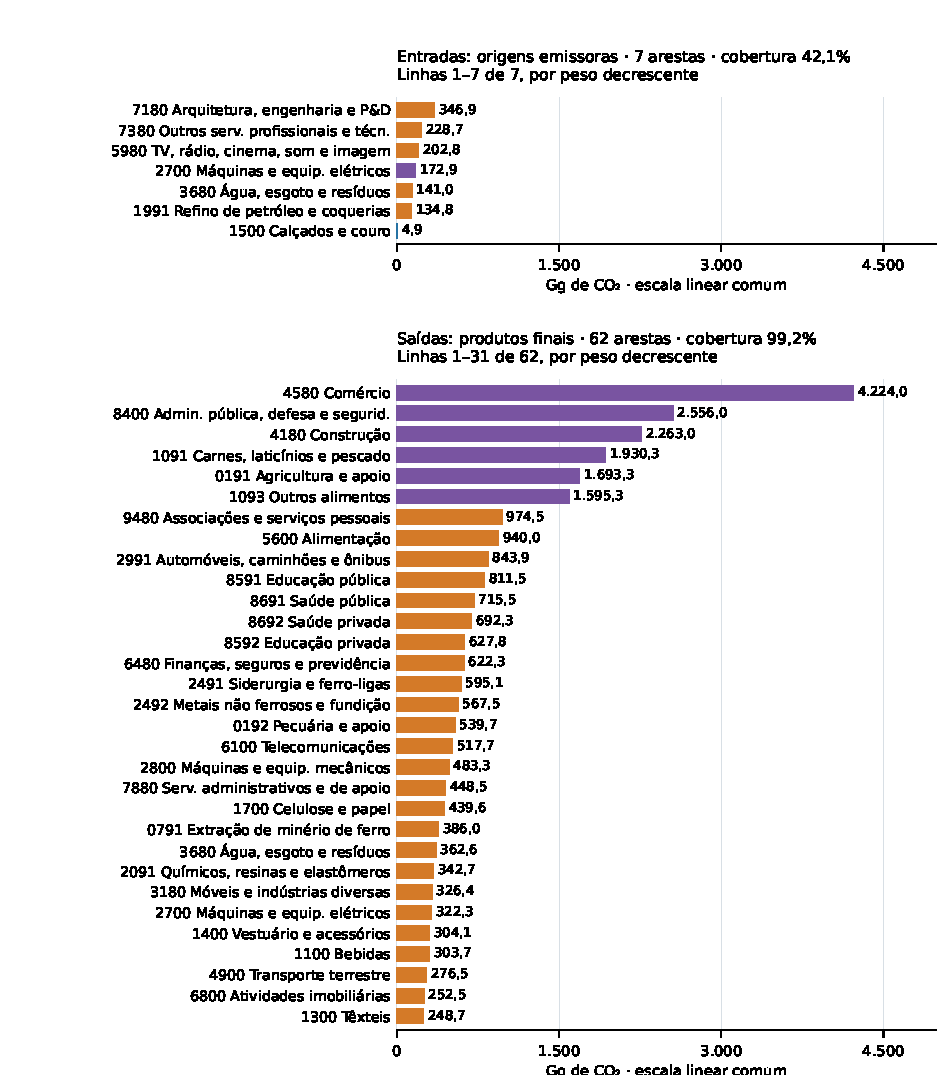
\includegraphics[width=\textwidth,height=0.78\textheight,keepaspectratio]{figuras/anexo_energia_1.pdf}
\caption{Energia (3500): todas as sete entradas e as saídas 1--31 de 62.}
\label{fig:anexo-energia}
\begin{minipage}{\textwidth}\footnotesize
Fonte: elaboração própria. Recortes de $\alpha=0{,}05$, com pesos originais em Gg de CO\textsubscript{2}, uma casa decimal e escala linear comum. A cobertura é o peso retido sobre a força da atividade e direção em $W$, sem diagonal: 42,1\% nas entradas e 99,2\% nas 62 saídas. As demais saídas aparecem na continuação, sem novo filtro. Azul: só saída na origem; laranja: só entrada no destino; roxo: ambos os testes.
\end{minipage}
\end{figure}
\clearpage
\begin{figure}[p]
\ContinuedFloat
\centering
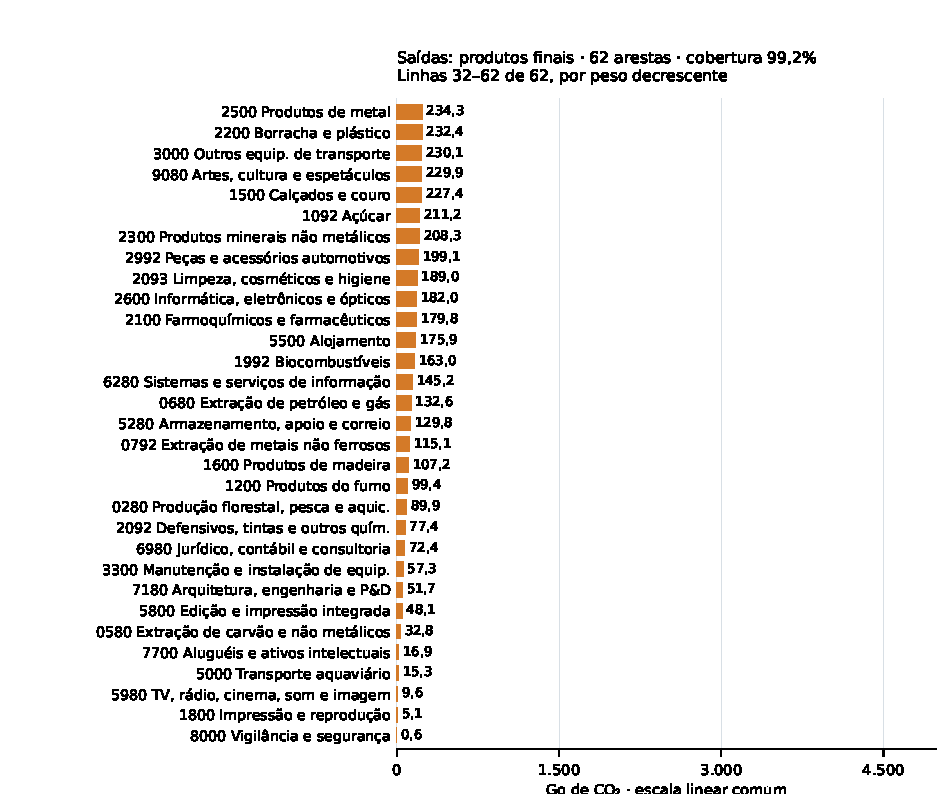
\includegraphics[width=\textwidth,height=0.85\textheight,keepaspectratio]{figuras/anexo_energia_2.pdf}
\caption{Energia (3500), continuação: saídas 32--62 de 62.}
\begin{minipage}{\textwidth}\footnotesize
Fonte: elaboração própria. Mesma seleção, ordem, escala e cores do painel anterior. A cobertura de 99,2\% se refere às 62 saídas, não apenas a esta página. Azul: só saída na origem; laranja: só entrada no destino; roxo: ambos os testes.
\end{minipage}
\end{figure}
\clearpage
\begin{figure}[p]
\centering
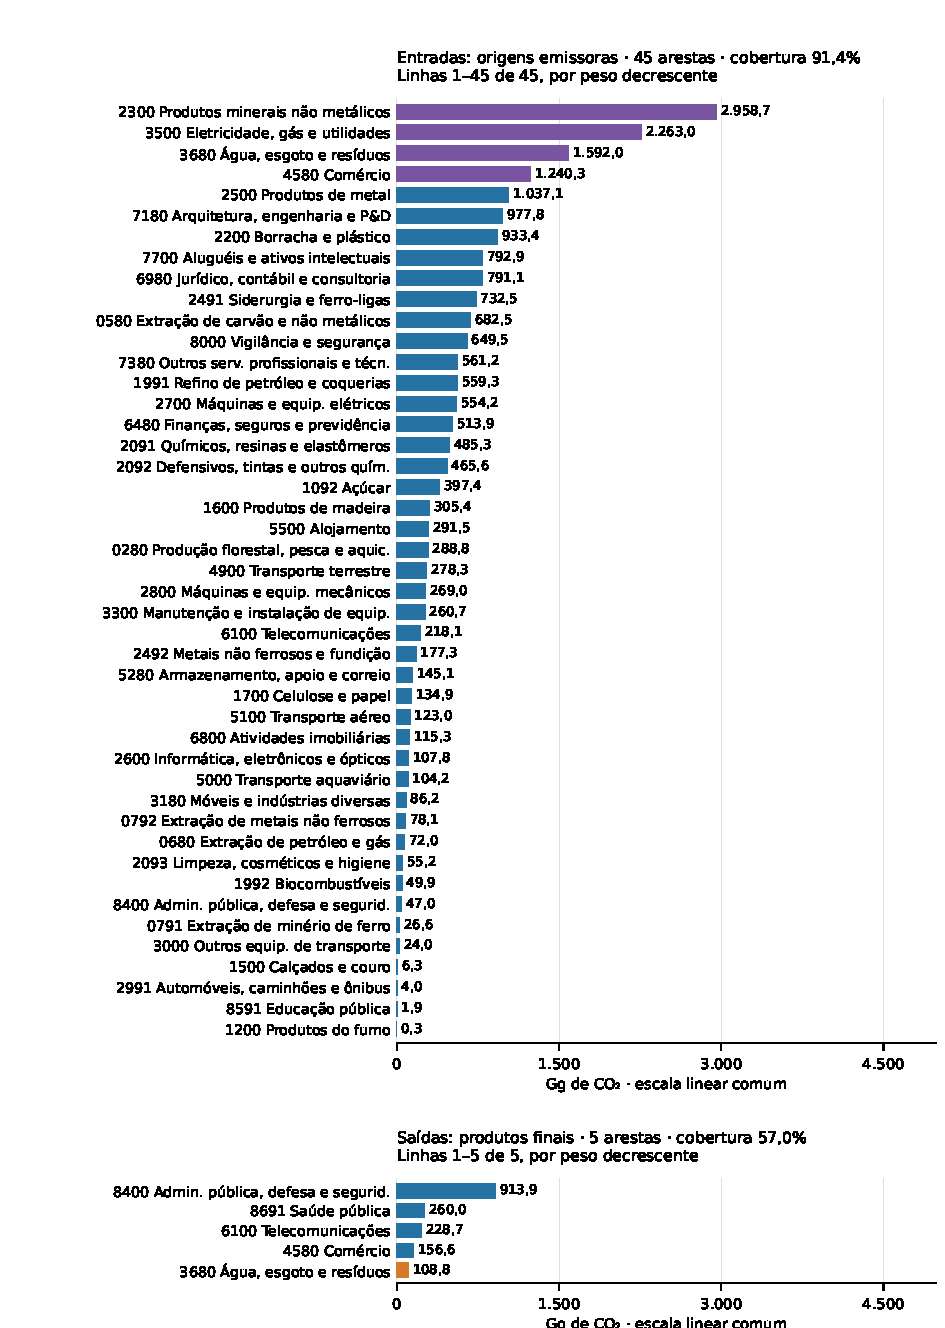
\includegraphics[width=\textwidth,height=0.85\textheight,keepaspectratio]{figuras/anexo_construcao.pdf}
\caption{Construção (4180): todas as 45 entradas e cinco saídas.}
\label{fig:anexo-construcao}
\begin{minipage}{\textwidth}\footnotesize
Fonte: elaboração própria. Coberturas de 91,4\% nas entradas e 57,0\% nas saídas. Mesma escala de pesos dos painéis de energia. Azul: só saída na origem; laranja: só entrada no destino; roxo: ambos os testes. Arestas compartilhadas não são duplicadas na rede.
\end{minipage}
\end{figure}
\clearpage

\section{Diagnósticos complementares da rede e da seleção}
\label{anexo:diagnosticos}

Na rede completa, os 66 perfis definidos têm medianas de 11,50 destinos efetivos e 13,93 origens efetivas, abaixo das 65 contrapartes existentes em cada direção. No backbone com $\alpha=0{,}05$, as medianas de cobertura são 59,32\% nas saídas e 55,69\% nas entradas.

A Tabela~\ref{tab:postos-complementares} detalha as mudanças de posição por grau em relação a $\alpha=0{,}05$. Os postos são calculados em ordem decrescente entre os 67 nós, com posto médio nos empates; reporta-se a mediana da mudança absoluta.

\begin{table}[htbp]
\centering
\caption{Mudança mediana de posição por grau em relação a $\alpha=0{,}05$.}
\label{tab:postos-complementares}
\begin{tabular}{@{}crr@{}}
\toprule
$\alpha$ & Grau de saída & Grau de entrada \\
\midrule
0,01 & 11 & 7 \\
0,10 & 4,5 & 4 \\
\bottomrule
\end{tabular}
\par\smallskip\begin{minipage}{\textwidth}\footnotesize
Fonte: elaboração própria. Valores em posições; as diferenças são calculadas a partir dos postos não arredondados, incluindo empates.
\end{minipage}
\end{table}

Dos 575 vínculos retidos em $\alpha=0{,}05$, 232 passam somente pelo teste de saída na origem, 265 somente pelo de entrada no destino e 78 pelos dois. Nenhum depende da convenção de grau um. A seleção por apenas uma extremidade mostra que uma relação pode destacar-se em um perfil sem ter a mesma importância relativa no outro.

Nos recortes da Tabela~\ref{tab:motivos-casos}, o backbone omite 57,9\% das entradas externas de energia e 43,0\% das saídas externas de construção. Esses complementos das coberturas evidenciam o volume omitido nas direções com menos ligações selecionadas.

\end{document}
